%!TEX TS-program = xelatex
% Исходная версия шаблона --- 
% https://www.writelatex.com/coursera/latex/5.1
\documentclass[c, dvipsnames]{beamer}  % [t], [c], или [b] --- вертикальное 
%\documentclass[handout, dvipsnames, c]{beamer} % Раздаточный материал (на слайдах всё сразу)
%выравнивание на слайдах (верх, центр, низ)
%\documentclass[handout, dvipsnames]{beamer} % Раздаточный материал (на слайдах всё сразу)
%\documentclass[aspectratio=169, dvipsnames]{beamer} % Соотношение сторон
\setbeamertemplate{navigation symbols}{}%remove navigation symbols

%\usetheme{Berkeley} % Тема оформленияLLL
%\usetheme{Bergen}
%\usetheme{CambridgeUS}
\usetheme{Boadilla}

\usecolortheme{crane} % Цветовая схема

%\useoutertheme{infolines} % Навигация 
%\useoutertheme{tree}
%\useoutertheme{miniframes}
%\useoutertheme{shadow}
%\useoutertheme{sidebar}
%\useoutertheme{smoothbars}
%\useoutertheme{smoothtree}
%\useoutertheme{split}
%\useoutertheme{default}


%\useinnertheme{circles}
\useinnertheme{rectangles}
%\useinnertheme{rounded}
%\useinnertheme{inmargin}


%%% Работа с русским языком
\usepackage[english,russian]{babel}   %% загружает пакет многоязыковой вёрстки
\usepackage{fontspec}      %% подготавливает загрузку шрифтов Open Type, True Type и др.
\defaultfontfeatures{Ligatures={TeX},Renderer=Basic}  %% свойства шрифтов по умолчанию
\setmainfont[Ligatures={TeX,Historic}]{Arial} %% задаёт основной шрифт документа
\setsansfont{Arial}                    %% задаёт шрифт без засечек
\setmonofont{Arial}
\usepackage{indentfirst}
\frenchspacing



%% Beamer по-русски
\newtheorem{rtheorem}{Теорема}
\newtheorem{rproof}{Доказательство}
\newtheorem{rexample}{Пример}

%%% Дополнительная работа с математикой
\usepackage{amsmath,amsfonts,amssymb,amsthm,mathtools} % AMS
\usepackage{icomma} % "Умная" запятая: $0,2$ --- число, $0, 2$ --- перечисление

%% Номера формул
\mathtoolsset{showonlyrefs=true} % Показывать номера только у тех формул, на которые есть \eqref{} в тексте.
%\usepackage{leqno} % Нумерация формул слева

%% Свои команды
\DeclareMathOperator{\sgn}{\mathop{sgn}}

%% Перенос знаков в формулах (по Львовскому)
\newcommand*{\hm}[1]{#1\nobreak\discretionary{}
{\hbox{$\mathsurround=0pt #1$}}{}}

%%% Работа с картинками
\usepackage{graphicx}  % Для вставки рисунков
\graphicspath{{images/}{images2/}}  % папки с картинками
\setlength\fboxsep{3pt} % Отступ рамки \fbox{} от рисунка
\setlength\fboxrule{1pt} % Толщина линий рамки \fbox{}
\usepackage{wrapfig} % Обтекание рисунков текстом

%%% Работа с таблицами
\usepackage{array,tabularx,tabulary,booktabs} % Дополнительная работа с таблицами
\usepackage{longtable}  % Длинные таблицы
\usepackage{multirow} % Слияние строк в таблице

%%% Программирование
\usepackage{etoolbox} % логические операторы

%%% Другие пакеты
\usepackage{lastpage} % Узнать, сколько всего страниц в документе.
%\usepackage{soul} % Модификаторы начертания
\usepackage{csquotes} % Еще инструменты для ссылок
\usepackage{multicol} % Несколько колонок


\usepackage{hyperref}
\usepackage{xcolor}
\hypersetup{        % Гиперссылки
    unicode=true,           % русские буквы в раздела PDF
    pdftitle={Заголовок},   % Заголовок
    pdfauthor={Автор},      % Автор
    pdfsubject={Тема},      % Тема
    pdfcreator={Создатель}, % Создатель
    pdfproducer={Производитель}, % Производитель
    pdfkeywords={keyword1} {key2} {key3}, % Ключевые слова
    colorlinks=true,        % false: ссылки в рамках; true: цветные ссылки
    linkcolor=,          % внутренние ссылки
    citecolor=green,        % на библиографию
    filecolor=magenta,      % на файлы
    urlcolor=blue           % на URL
} 

\usepackage{dcolumn}

%fffff3
\definecolor{backgr}{RGB}{146,26,29}
\definecolor{backgr1}{RGB}{230,43,37}
\definecolor{ex1}{RGB}{231,142,36}
\definecolor{ex2}{RGB}{249,155,28}
\definecolor{ex3}{RGB}{242,103,36}

\definecolor{red}{RGB}{230,43,37}
%\setbeamercolor{normal text}{fg=black,bg=backgr}
\setbeamercolor{frametitle}{bg=backgr,fg=white}
%\setbeamercolor{footline}{bg=backgr,fg=white}
%\setbeamercolor{normal text}{bg=yellow}
%\setbeamercolor{section in toc}{fg=yellow}
%\setbeamercolor{subsection in toc}{fg=blue}

% How to change colour of Navigation Bar in Beamer -  много интересного

%Пример команд, задающих внешний вид блока
\setbeamercolor{block title}{fg=white,bg=ex1}
\setbeamerfont{block title}{family=\sffamily}
\setbeamercolor{block body}{bg=white}
\setbeamertemplate{blocks}[rounded][shadow=fasle]
\setbeamercolor{title}{bg=backgr, fg=white}
\setbeamercolor{alerted text}{fg=backgr1}

\newlength\subtitwd
\setlength\subtitwd{4cm}% change the width here

\makeatletter
\newcommand\titlegraphicii[1]{\def\inserttitlegraphicii{#1}}
\titlegraphicii{}



%\newcommand\superviser[1]{\def\insertsuperviser{Научный руководитель: #1}}
\newcommand\superviser[1]{\def\insertsuperviser{  #1}}



\superviser{}

\setbeamertemplate{title page}
{
  \vbox{}
   {\usebeamercolor[fg]{titlegraphic} \hspace{0.35ex} \inserttitlegraphic\hfill\inserttitlegraphicii \hspace{1ex} \par }\vspace{1.5ex}
  \begin{centering}
    \begin{beamercolorbox}[sep=8pt,center]{institute}
      \usebeamerfont{institute}\insertinstitute
    \end{beamercolorbox}
    \begin{beamercolorbox}[sep=8pt,center]{title}
    
      \usebeamerfont{title}\inserttitle\par%
      \ifx  \insertsubtitle\@empty%
      \else%
        \vskip0.5em%
        {\usebeamerfont{subtitle}\usebeamercolor[fg]{subtitle}\insertsubtitle\par}%
      \fi%     
    \end{beamercolorbox}%
    \vskip1em\par
    \begin{beamercolorbox}[sep=5pt,center]{date}
      \usebeamerfont{date}\insertdate
    \end{beamercolorbox}%\vskip0.5em
    \begin{beamercolorbox}[sep=5pt,center]{author}
      \usebeamerfont{author}\insertauthor
    \end{beamercolorbox}
        \begin{beamercolorbox}[sep=4pt,center]{institute}
      \usebeamerfont{institute}\insertsuperviser
    \end{beamercolorbox}
  \end{centering}
  %\vfill
}
\makeatother

\setbeamercolor{item projected}{bg=ex3}
\setbeamertemplate{enumerate items}[default]

\setbeamercolor{palette primary}{bg=white}
\setbeamercolor{palette primary}{fg=black}
\setbeamercolor{palette secondary}{bg=white}
\setbeamercolor{palette secondary}{fg=black}
\setbeamercolor{palette tertiary}{bg=white}
\setbeamercolor{palette tertiary}{fg=black}

\setbeamercolor{itemize item}{fg=ex3}
\setbeamercolor{itemize subitem}{fg=ex2}
\setbeamercolor{itemize subsubitem}{fg=ex1}

\setbeamercolor{enumerate item}{fg=ex3}
\setbeamercolor{enumerate subitem}{bg=ex3}
\setbeamercolor{enumerate subsubitem}{bg=ex3}


\setbeamertemplate{itemize subitem}{$\Rightarrow$}
\setbeamertemplate{itemize item}{$\blacktriangleright$}



\usepackage{todo}
\newcolumntype{a}{>{\columncolor{red}}c}


\usefonttheme{professionalfonts}

\title[   Моделирование цен на электричество ]{Моделирование спотовых цен на электроэнергию    на оптовом рынке  в России }
%\subtitle{Защита выпускной квалификационной работы}


%Stochastic Factors Affecting Commodity Prices: the Case of Russia

\usepackage{amsmath}
\usepackage{ragged2e}

\author[Касьянова Ксения]{Докладчик: Касьянова Ксения \\ \smallskip  \href{mailto:kasyanova-ka@ranepa.ru}{kasyanova-ka@ranepa.ru}   \bigskip \scriptsize }

\superviser{ Руководитель НИР: Каукин А.С., к.э.н, зав. лабораторией \\ \smallskip   НИР в рамках исполнения Государственного задания \\ РАНХиГС при Президенте Российской Федерации на 2020 год}

%\author[Имя автора]{Имя автора \\ \smallskip \scriptsize \href{mailto:author@ranepa.ru}{author@ranepa.ru} \\ \smallskip  \href{http://ranepa.ru}{http://ranepa.ru} }

\institute[ИОРИ РАНХиГС]{ \uppercase{
  Институт отраслевых рынков и инфраструктуры} \\ \smallskip   Лаборатория системного анализа
отраслевых рынков }
\date{}



\titlegraphic{
\includegraphics[scale=0.5]{logo1}}
\titlegraphicii{
\includegraphics[scale=0.5]{logo2}}

\usepackage[figurename= ]{caption}

\begin{document}

\frame[plain]{\titlepage}	% Титульный слайд


\section{Введение}

\begin{frame}[shrink=3]

\frametitle{Общие сведения о выполняемой НИР} 

\footnotesize

\begin{block}{Мотивация:}
	\begin{itemize}		
		\item экономические модели требуют введения определенных предпосылок и упрощений;
		\item при моделировании цены как случайного процесса не учитываются экономические факторы.
%		\item  
%		моделирование цены на оптовом рынке электроэнергии как случайного процесса с учётом особенностей российского рынка. 		
	\end{itemize}
\end{block}

\begin{block}{Цель работы:}
\begin{itemize}
	\item разработка модели, учитывающей недостатки двух классов моделей:    моделирование цены на оптовом рынке электроэнергии как диффузионно-скачкообразного процесса  с учётом фундаментальных факторов спроса и предложения (температура, уровень деловой активности и др.),  особенностей российского рынка. 		
\end{itemize}
\end{block}



\begin{block}{Гипотеза:}
	\begin{itemize}
		\item с помощью построенной модели можно получить трендсезонное разложение цены на электричество с более точными оценками коэффициентов при интересующих нас переменных. 
		%		\item стандартные модели оценки риска не подходят для российской рынка, риск недооценен, добавление дополнительных факторов позволит получить более точные оценки риска. 	
	\end{itemize}
\end{block}

\end{frame}

%		\item оценка влияния принятия различных решений  и финансовые риски участников рынка электрической энергии. 
%модель строится с целью иметь возможность проследить, что произойдет на рынке при влиянии на какие-то из встроенных в модель факторов
% надо понимать, что без учета стохастической компоненты это невозможно, так как цена на эл-во нестанционарный процесс и при оценке  какого-либо  влияния факторов на цены велика вероятность, что колебания в этот момент были случайными  

% боремся с этим, во-первых, добавляя в модель стохастическую компоненту, во-вторых, используя байесовский подход при оценке этой модели мы сможем получить результат в виде "с какой вероятностью такие изменения на рынке были вызваны именно внешний воздейтсвием на фактор, а не случайными изменениями цены"

\begin{frame}[shrink=5]
\frametitle{Результаты работы могут быть использованы:} 

\footnotesize{
%\begin{block}{Результаты работы могут быть использованы:}
	\begin{itemize}
		
%		\item совершенствование метода статистического анализа случайных процессов;
		\item для научно-методологического обеспечения прикладных исследований и моделирования рынков электроэнергии, в частности совершенствования методов статистического анализа случайных процессов;
		\item для разработки конкретных направлений, мер и механизмов государственной политики в сфере регулирования рынка электроэнергии:
%		\item модель тренд-сезонного разложения полезна при разработке предложений по изменению и дополнению нормативных правовых актов регулирующих рынок  электроэнергии. 
		%		 позволит оценить влияние изменения экономических факторов на каждую из компонент тренд-сезонного разложения. 
		\begin{figure}
			\centering
			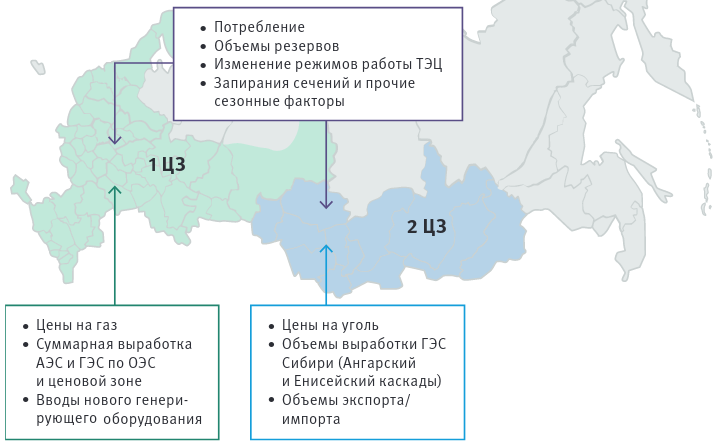
\includegraphics[width=0.6\linewidth]{screenshot034}
			\label{fig:screenshot033}
		\end{figure}
				\begin{itemize}
					\footnotesize{
					\item определение темпа роста цен на электроэнергию; 
					\item причины различия в динамике цен в ценовых зонах;
					\item влияние структуры генерирующих мощностей на волатильность цен;
					\item оценка влияния резких изменений экономических факторов на цены.  }
				\end{itemize}
	\end{itemize}
%\end{block}
}
%\begin{block}{Примеры:}
%	\begin{itemize}
%		\item  возможность детального анализа финансовых рисков на рынке электричества необходима при  проведении  социально- экономической политики  и разработке предложений по изменению и дополнению нормативных правовых актов регулирующих рынок  электроэнергии:
%		\begin{itemize}
%			\footnotesize{
%			\item определение темпа роста цен на электроэнергию; 
%			\item причины различия в динамике цен в ценовых зонах;
%			\item влияние структуры генерирующих мощностей на волатильность цен;
%			\item оценка влияния резких изменений экономических факторов на цены.  }
%		\end{itemize}
		% диверсификация рисков, при определении будет ли удовлетворен спрос		
		% необходимость верно оценивать финансовые риски возникает у производителей электричества; (1 час - 1 день),    финансовых посредников  торгующих контрактами на электроэнергию (1 день - 1 месяц), инвесторов (1 месяц - 1 год).
		% прямая связь с задачей ценообразования производных финансовых инструментов, необходимых для хеджирования  финансовых рисков. фьючерсы недавно торгуются, в России биржа электричества молодая, Россия необычная страна).  
%	\end{itemize}
%\end{block}


%	\item причины энергетических кризисов: изменения налогообложения, рыночные манипуляции, устаревшая инфраструктура, провалы рынка, излишняя зарегулированность, перебои с поставками топлива, резкое изменение климата,  доставка электричества дешевле стоимости производства 

\end{frame}


\begin{frame}[shrink=3]
\frametitle{Задачи} 

\footnotesize{
%\begin{block}{Задачи:}
	\begin{itemize}
%		\item  описание принципа функционирования оптового рынка электроэнергии;
		\item  определение факторов влияющих на цены на электричество, особенностей российского рынка; 	
		\item  выбор подходящей модели, способной учесть неодинаковое    влияние факторов на различные компоненты процесса (тренд, сезонность и стохастические компоненты);
		\item  оценивание моделей, сравнение с моделями не учитывающими стохастические компоненты, моделями оцененными на данных, очищенных от выбросов;
		\item  сравнение финансовых рисков до/после событий, влияющих на факторы, включенные в модель. 
%		\item  сравнение классических моделей оценки риска (VaR) на российских данных (можно попробовать применить к американским/европейским);		
%		цель посчитать VaR в класическом  варианте, сравнить с реальными рисками, сказать, что риск был недоценен, улучшить с помощью изменения распределения				  		
%		  цены и оценка риска на российском рынке электричества с учетом этих факторов, сравнение с классической моделью,  выявление причин, по которым  в какие-то моменты риски были завышены/занижены.
% 		\item  проверка коинтегрированности факторов с ценами;
%		\item  добавление факторов в модели оценки риска (например, вместо нормального распределения в VaR моделях использовать скорректированное распределение, учитывающее эти факторы);
%\item  сравнение модели с базовыми: определить, удалось ли решить проблему с неправильными оценками риска. 				
	\end{itemize}
}
%\end{block}

\end{frame}


\begin{frame}[shrink=5]
\frametitle{Содержание} 
\begin{enumerate}
	\item Способы моделирования цен на электричество:
	\begin{enumerate}
		\item экономические модели; 
		\item случайные процессы.
%		моделирование цены как диффузионно-скачкообразного процесса.		
	\end{enumerate}
	\item Выбор факторов, влияющих на цены:
	\begin{enumerate}
		\item особенности рынка электричества;
		\item принцип работы ОРЭМ и особенности российского рынка;
		\item выбор ценовых факторов, включаемых в модель.
	\end{enumerate}
	%	\item моделирование цены как диффузионно-скачкообразного процесса + экономические факторы
\end{enumerate}
\end{frame}



\section{Модель}

\begin{frame}[shrink=5]

%\frametitle{Факторы  влияющие на цены на электричество} 

\frametitle{Классификация моделей} 

\begin{figure}
	\centering
	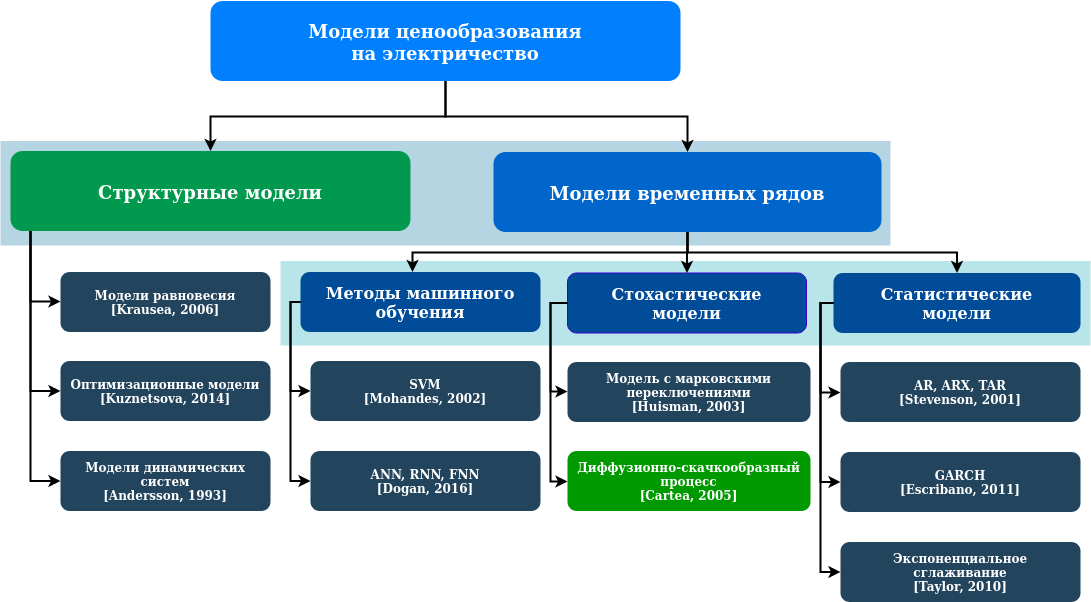
\includegraphics[width=1\linewidth]{untitled2}
	\label{fig:untitled-diagram}
\end{figure}


\end{frame}




\begin{frame}[shrink=5]
\frametitle{Анализ предметной отрасли} 
\begin{table} \small\centering\setlength{\extrarowheight}{0.25em}
	
	\begin{tabular}{   >{\centering\scriptsize}p{3cm} 
			>{\centering\scriptsize}p{3.5cm}
			>{\RaggedRight\scriptsize\arraybackslash}p{5cm} }\hline		
		Авторы, год & Название работы &  Результат \\\hline 
		%		Mehdi Sadeghi, Saeed Shavvalpour (Energy Policy, 2006) & \href{https://www.researchgate.net/publication/222400423_Energy_risk_management_and_value_at_risk_modeling}{Energy risk management and value at risk modeling}  &     \\
		Judio Lucia, Eduardo Schwartz (Review of Derivatives Research, 2002) & \href{https://link.springer.com/article/10.1023\%2FA\%3A1013846631785}{Electricity Prices and Power Derivatives: Evidence from the Nordic Power Exchange}  &   Эмпирическая оценка детерминистической сезонной компоненты   в одно- и двухфакторной модели  цен на электричество.  \\
		Álvaro Cartea, Marcelo G. Figueroa (Applied Mathematical Finance, 2005) & \href{https://www.researchgate.net/publication/24071715_Pricing_in_Electricity_Markets_A_Mean_Reverting_Jump_Diffusion_Model_with_Seasonality}{Pricing in Electricity Markets: a mean reverting
			jump diffusion model with seasonality}  &   Применение  модели цен на электричество,  учитывающую тенденцию возвращения к среднему, скачкообразность и сезонность процесса.    \\	
		Maciej Kostrzewski, Jadwiga Kostrzewska (Energy Economics, 2019) & \href{https://www.researchgate.net/publication/331065098_Probabilistic_Electricity_Price_Forecasting_with_Bayesian_Stochastic_Volatility_Models}{Probabilistic Electricity Price Forecasting with Bayesian Stochastic Volatility Models}  &   Прогнозирование спот-цен на электричество с помощью  байесовского подхода  позволяет учесть  неопределенность в распределении коэффициентов параметров, что улучшает прогнозы в сравнении с классическими моделями.  
		%		L. YANG, S. HAMORI (2018) & \href{https://www.worldscientific.com/doi/abs/10.1142/S2010495218500100}{MODELING THE DYNAMICS OF INTERNATIONAL AGRICULTURAL COMMODITY PRICES:A COMPARISON OF GARCH AND SV MODELS}  &    Основываясь на ежемесячных данных, скачкообразные процессы и асимметричный эффект не влияют на цены на сельскохозяйственную продукцию. Оценивая VaR для этих сельскохозяйственных товаров, мы обнаруживаем, что резкий рост цен на сельскохозяйственную продукцию в 2008 году мог быть вызван частой перебалансировкой портфелей. \\
		%		 
		%статья напечатана в говножурнале. Я бы не стал ориентироваться на такое.	
		%		Mária Bohdalová, Michal Greguš (2015) & \href{https://www.researchgate.net/publication/283243124_ESTIMATING_VALUE-AT-RISK_BASED_ON_NON-NORMAL_DISTRIBUTIONS}{ESTIMATING VALUE-AT-RISK BASED ON NON-NORMAL DISTRIBUTIONS}  &    Моделирование VaR в предположении, что ежедневные изменения цен iid не с нормальным распределением или   автокоррелированны  с через  динамику факторов риска \\
		%  это похоже на пересказ учебника,  к науке и постановке вопроса оно имеет весьма опосредованное отношение.
		%		Rainer Göb (2011) & \href{https://onlinelibrary.wiley.com/doi/abs/10.1002/qre.1238}{Estimating value at risk and conditional value at risk for count variables}  &    Эмпирические аспекты оценки риска с биномиальным распределением и распределении Пуассона. Особое внимание уделяется интервальной оценке мер риска.  \\\hline 	
		%			H. Mostafaei et al.  (2013) & 
		%		\href{https://dergipark.org.tr/en/download/article-file/361215}{A Methodology for the Choice of the Best Fitting Continuous-Time Stochastic Models of Crude Oil Price: The Case of Russia }   & Выбор стохастического процесса наилучшим образом, описывающего цену на нефть \\
		%			 A. Murat,  E. Tokat (2009) & \href{https://www.sciencedirect.com/science/article/pii/S0140988308001096?via\%3Dihub}{Forecasting oil price movements with crack spread futures}
		%			   &   Коинтегрированность цен  на нефть и фьючерсов на крэк-спред => прогнозы VECM with crack spread futures лучше, чем у VECM with crude oil futures. 
	\end{tabular}
\end{table}
\end{frame}

\begin{frame}[shrink=5]
\frametitle{ Модель Мертона (Merton’s Jump-Diffusion Model) } 

\begin{block}{Kostrzewski and Kostrzewska (2019): }

Базовая модель описывающая цену на электричество: 

\footnotesize{
\begin{itemize}
	\item эмпирическое распределение имеет тяжелые хвосты, что не согласуется со стандартной моделью Блэка-Шоулза
	\item  в модель добавляется отдельная компонента, отвечающая за скачкообразность процесса. 
\end{itemize}
}

Риск-нейтральный диффузионно-скачкообразный процесс (jump-diffusion process), описывающий изменение цены на электричество $S_t$:

$$dS_t/S_t=(r−\lambda \bar{k})dt+\sigma dW_t+kdq_t,$$

\begin{itemize}
	\item где $\sigma$ - волатильность диффузионной компоненты, при  $\lambda=0$ получаем модель Блэка-Шоулза;
\item cкачки порожденны составным процессом Пуассона  $q_t$  с параметром  $\lambda$, где $k$  - величина случайного скачка (логнормально распределенный):    
$$ln(1 +k)\sim N(\gamma,\delta^2)$$
\item где среднее - $\bar{k} = E(k)=e^{\gamma + \delta^2/2}-1$.

\end{itemize}

\end{block}

\end{frame}

\begin{frame}[shrink=5]
\frametitle{Модели с детерминистической компонентой} 

\begin{block}{Lucia and Schwartz (2002): }

Модели с детерминистической сезонной компонентой:   

-- однофакторная модель спотовых цен: 	
	\begin{align*}
	 ln (S_t) & = f(t) + X_t \\
	dX_t & = -\kappa X_t dt + \sigma(t) dW
	\end{align*}
-- двухфакторная модель спотовых цен: 	
\begin{align*}
ln (S_t) & = f(t) + X_t + \epsilon_t\\
dX_t & = -\kappa X_t dt + \sigma_X(t) dW_X\\
d\epsilon_t & = \mu_{\epsilon}  dt + \sigma_{\epsilon}(t) dW_{\epsilon}\\
dW_X dW_{\epsilon} &= \rho dt
\end{align*}
\footnotesize{
где  $g(t) = e^{f(t)}$ - детерминистическая функция сезонности, $X_t$ - процесс, возвращающий среднее (OU process) с нулевым долгосрочным средним и скоростью подстройки $\kappa$.}
	%Эмпирическая оценка детерминистической сезонной компоненты   в одно- и двухфакторной модели  цен на электричество. 
\end{block}

%Применение  модели цен на электричество,  учитывающую тенденцию возвращения к среднему, скачкообразность и сезонность процесса.

%\begin{block}{Cartea and Figueroa (2005): }
%	$Y_t$ - диффузионно-скачкообразный процесс:
%	
%	$$dY_t = -\alpha Y_t dt + \sigma(t) dW_t + J dq_t$$
%	
%	$J$ - величина скачка, $q$ - пуассоновский процесс.
%\end{block}
\end{frame}




\begin{frame}[shrink=5]
\frametitle{Kostrzewski and Kostrzewska (2019)} 

\textbf{Модель стохастической волатильности с экспоненциально распределенными скачками, эффектом рычага и экзогенными переменными  (SVDEJX*):
}


\begin{itemize}

	\item  для прогнозирования используется SV модель с экзогенными переменными (температура) и дамми-переменными на выходные и понедельник;
	\item  в модели скачки вверх/вниз распределены экспоненциально, с разными параметрами;
		$$  \xi_{ t}^U \sim Exp(\eta_U) \ i.i.d., \xi_{ t}^D \sim Exp(\eta_D) \ i.i.d.$$
	\item  с помощью байесовского подхода можно оценить ненаблюдаемые компоненты модели $\xi_{ t}^U, \xi_{ t}^D, q_{t}, h_{ t}$:
	
\begin{equation}\label{key}
	q_{ t} =\begin{cases} \ 1, \ \ \ \  p_D\\ \ 0, \ \ \ \   p_0  \\ -1, \ \ \ p_U 
\end{cases}
\end{equation}	

\end{itemize}

* Stochastic
	volatility model with a double exponential distribution of jumps, a leverage
	effect and exogenous variables. 



\end{frame}

\begin{frame}[shrink=5]
\frametitle{Kostrzewski and Kostrzewska (2019)} 

Модель стохастической волатильности SVDEJX: 
\begin{align*}
y_{t} = y_{ t-1} & + \mu + \psi X_{ t }+ d_{ Sat} D_{ Sat,t} + d_{ Sun }D_{ Sun,t} + d_{ Mon }D_{ Mon,t} +  \\ & + \sqrt{exp(h_{ t-1} )}\epsilon_{ t }^{(1)}+ J _{t }\\
h_{t-1} &= h_{ t-2} + \kappa_{ h} (\theta_{ h} - h_{ t-2} ) + \sigma_{ h} (\rho \epsilon_{ t-1}^{(1)} + \sqrt{1 - \rho^2} \epsilon_{ t-1}^{(2)}) \\
J_{ t} &= -\xi_{ t}^D \cdot \mathbb{I}(q_{ t} = -1) + 0 \cdot \mathbb{I} (q_{ t} = 0) + \xi_{ t}^U \cdot \mathbb{I} (q_{ t} = 1)
\end{align*}

\footnotesize{
\begin{itemize}


	\item $y_{ t} = ln(S_{ t})$ --  логарифм цены

\item  $h_{t-1} = y_{t} - y_{ t-1}$ 


\item  $X_{ t}$ -- логарифм почасовой температуры

\item  $D_{ Sat, t}, D_{ Sun, t}, D_{ Mon, t}$  -- учитывают недельную сезонность

\item $q_{t}$ -- наличие скачка вверх/вниз (значения переменной ненаблюдаемы, но можно оценить вероятность скачка)


\item  $\rho < 0$ -- параметр ''рычага'', $\rho > 0$ -- обратный параметр ''рычага'' (если большим значениям логарифма цены  соответствуют большие значения дисперсии)

\item  $\epsilon_{ t }^{(1)}, \epsilon_{ t }^{(2)} \sim N(0,1) \ i.i.d.$, $\xi_{ t}^D \sim Exp(\eta_D) \ i.i.d. $,  
$\xi_{ t}^U \sim Exp(\eta_U) \ i.i.d.$


\end{itemize}

}
\end{frame}



\begin{frame}[shrink=5]
\frametitle{Kostrzewski and Kostrzewska (2019)} 

Данные: 
\begin{itemize}
	\item Спотовые цены JCPL (Jersey Central Power and Light Company), находящейся   в первой  ценовой зоне, определяемой сетевым оператором PJM Interconnection.
	\item Период: 22/08/2010 ---  14/01/2012
\end{itemize}

\begin{figure}
\centering
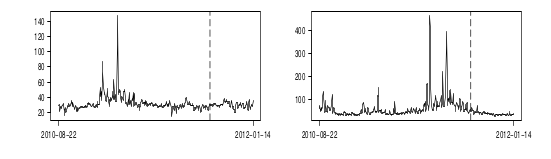
\includegraphics[width=1\linewidth]{screenshot012}
\caption{Спотовые цены на 4 часа (непиковый час) и 16 часов (пиковый час), USD/MWh }
\label{fig:screenshot006}
\end{figure}

\end{frame}





\begin{frame}[shrink=5]
\frametitle{Kostrzewski and Kostrzewska (2019)} 
\begin{figure}
\centering
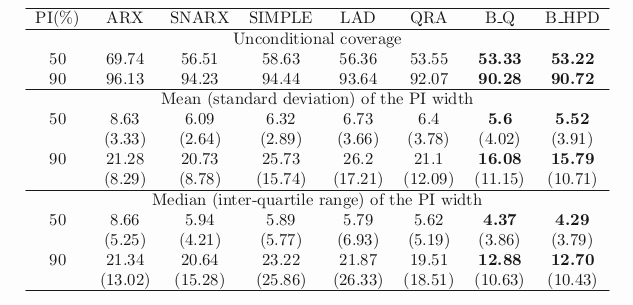
\includegraphics[width=0.9\linewidth]{screenshot006}
\caption{Сравнение ширины доверительных интервалов прогноза, полученных по байесовским (B\_Q, B\_HPD) и не байесовским моделям. Результат получен по данным за все 24 часа.}
\label{fig:screenshot006}
\end{figure}
\end{frame}





\section{Российский рынок}

\begin{frame}[shrink=5]

%		\item около 72\% производимой электроэнергии продается на рынке на сутки вперед (РСВ);
\frametitle{Российский рынок электроэнергии и мощности} 
\begin{figure}
	\centering
	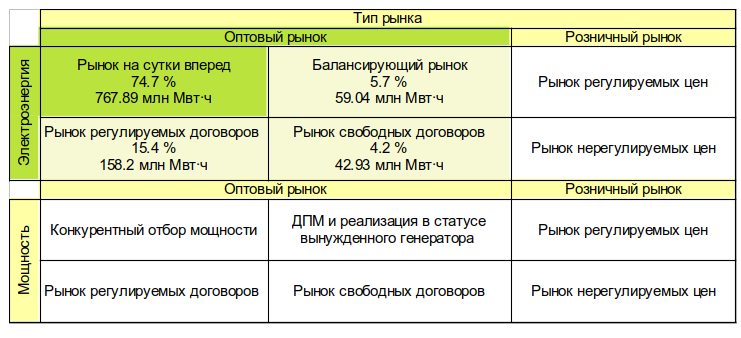
\includegraphics[width=0.9\linewidth]{screenshot023}
	\caption{Классификация рынков электроэнергии и мощности России}
	\label{fig:screenshot004}
\end{figure}


\footnotesize{(*) Структура объемов реализации электрической энергии в секторах оптового рынка электроэнергии за 2016 г. 

%https://www.ruscable.ru/article/Electric_power_industry_of_Russia/

(**) Потребление электроэнергии по субъектам Российской Федерации в 2016 г --  1077.94 млн.МВт.час. Росстат
}




\end{frame}




\begin{frame}[shrink=5]
\frametitle{Российский оптовый рынок электричества} 
\begin{figure}
	\centering
	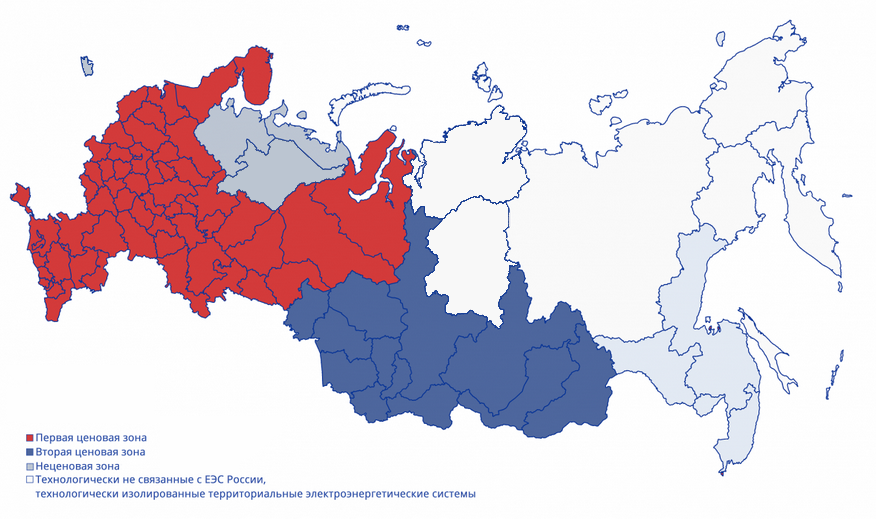
\includegraphics[width=1\linewidth]{screenshot014}
	\caption{ Ценовые зоны. Источник: АТС }
	\label{fig:screenshot013}
\end{figure}
\end{frame}








\begin{frame}[shrink=5]
\frametitle{Российский рынок электроэнергии и мощности} 
\framesubtitle{Формирование тарифа для конечного потребителя на электроэнергию} 

%Тариф для конечного потребителя на электроэнергию и мощность формируется на основе пяти составляющих:

\footnotesize{
\begin{itemize}
	\item цена покупки электроэнергии на оптовом рынке или у розничного генератора;
	\item  цена покупки мощности энергосбытовой компанией на оптовом рынке или у розничного генератора;
	\item  цена передачи по сети с дифференциацией по уровню напряжения;
%	 тарифы ФСК на передачу по магистральным сетям, тарифы МРСК на передачу по сетям среднего напряжения и тариф ТСО на передачу по сетям низкого напряжения;
	\item  инфраструктурные платежи: плата за услуги СО ЕЭС, АТС, ЦФР; 
%	Размер платы регулируется ФАС Россиии Ассоциацией «НП Совет рынка»;
	\item  надбавка сбытовых компаний  (кроме участников оптового рынка).
	
\end{itemize}
} 


\begin{figure}
	\centering
	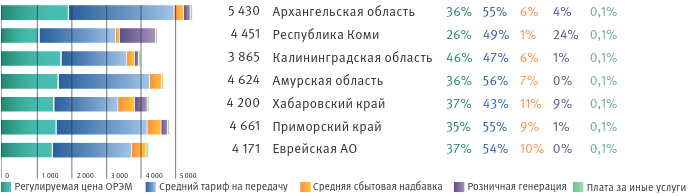
\includegraphics[width=0.7\linewidth]{screenshot024}
	\caption{Средневзвешенные регулируемые цены на электрическую энергию для потребителей первой ценовой категории за 2017 год, руб./МВт.ч }
	\label{fig:screenshot024}
\end{figure}

Источник: ''НП Совет Рынка''

\end{frame}


\begin{frame}[shrink=5]
\frametitle{Российский оптовый рынок электричества} 
\framesubtitle{Формирование кривой совокупного предложения }
%\begin{figure}
%	\centering
%	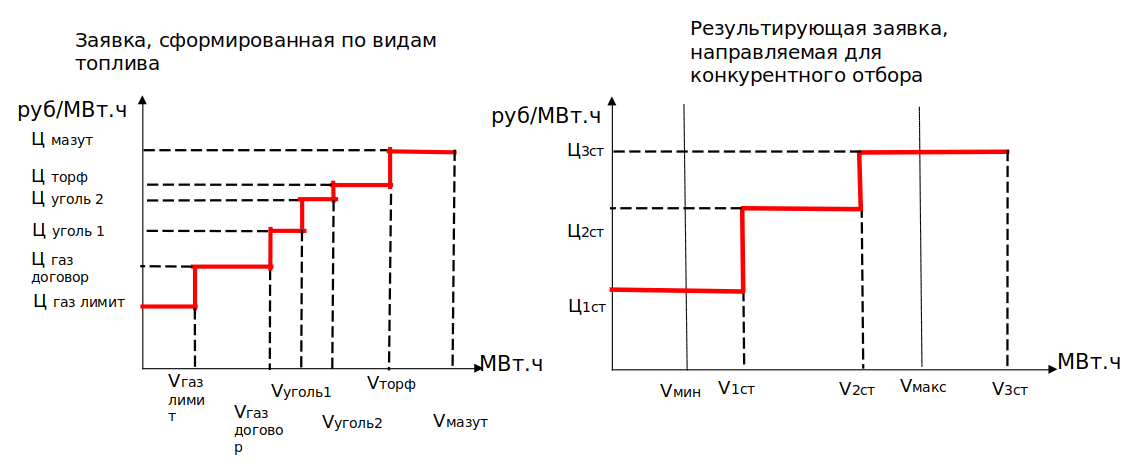
\includegraphics[width=0.7\linewidth]{screenshot016}
%	\caption{Формирование ценовой заявки поставщика 
%		для конкурентного отбора  РСВ и БР. Источник: E.ON  }
%	\label{fig:screenshot016}
%\end{figure}
\vfil
\hfil\hfil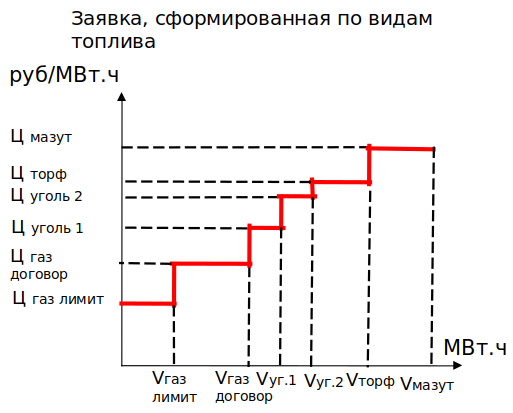
\includegraphics[height=3.5cm]{screenshot030}\hfil\hfil
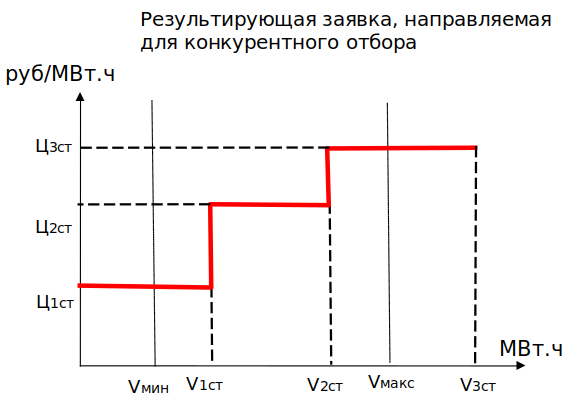
\includegraphics[height=3.5cm]{screenshot031}
\newline
\vfil
\hfil\hfil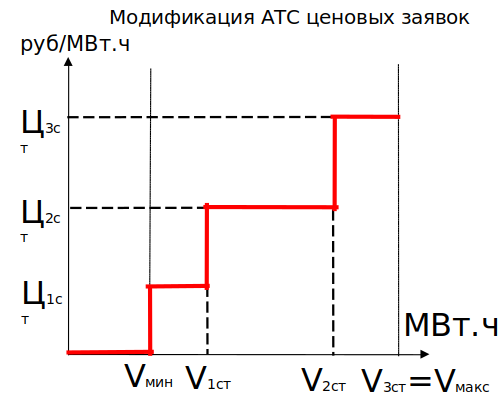
\includegraphics[height=3.5cm]{screenshot027}\hfil\hfil
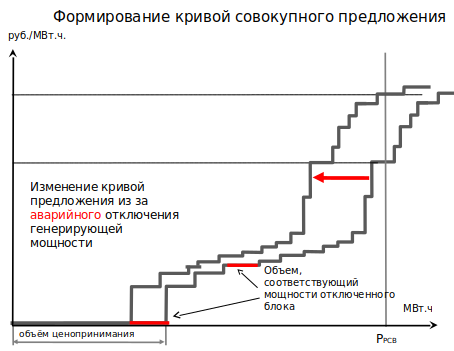
\includegraphics[height=3.5cm]{screenshot029}
\newline
\footnotesize{Источник:  ОАО ''Э.ОН Россия'' }

\end{frame}



\begin{frame}[shrink=5]
\frametitle{Российский оптовый рынок электричества} 

\begin{figure}
\centering
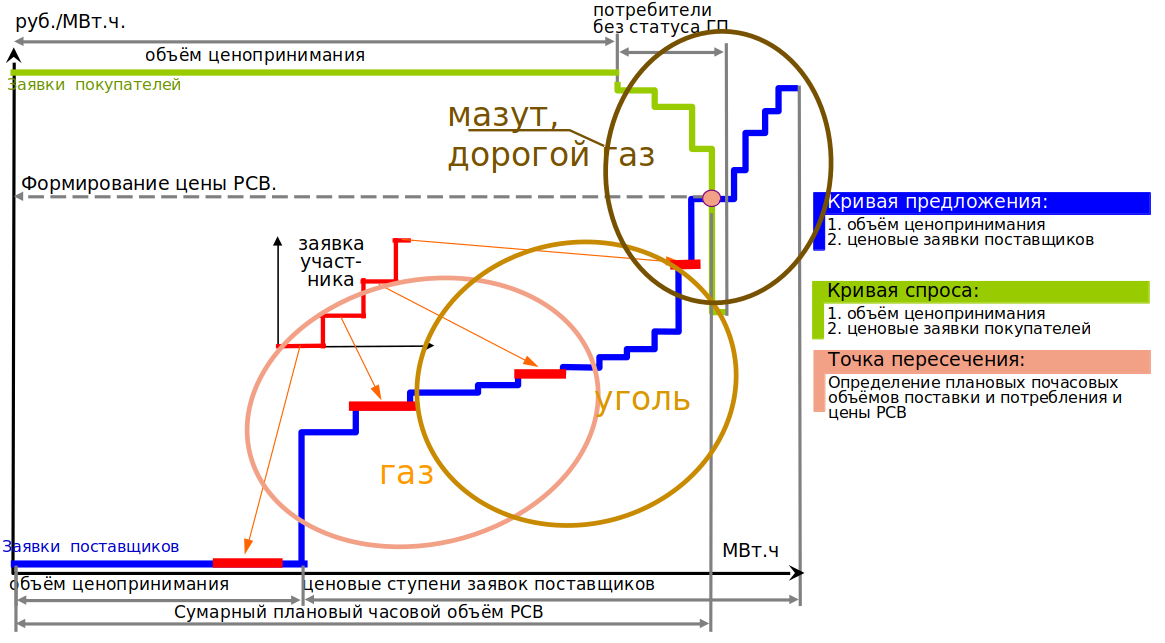
\includegraphics[width=1\linewidth]{screenshot032}
\caption{ Определение и фиксация объемов поставки и потребления.  Источник: ОАО ''Э.ОН Россия'' }
\label{fig:screenshot015}
\end{figure}

\end{frame}








\begin{frame}[shrink=5]
\frametitle{Данные} 


Данные по ценам на электричество за каждый час, начиная с 1.08.2013 по двум ценовым зонам (источник: \href{https://www.atsenergo.ru/results/rsv}{АТС}).

\begin{itemize}
	\item Индекс равновесных цен на покупку электроэнергии, руб./МВт.ч.
	\item Объем полного планового потребления, МВт.ч
%	\item Объем покупки по регулируемым договорам, МВт.ч
	\item  Объем покупки на РСВ, МВт.ч	
%	\item Объем продажи в обеспечение РД, МВт.ч	
	%	\item  Максимальный индекс равновесной цены, руб./МВт.ч	\item Минимальный индекс равновесной цены, руб./МВт.ч
	%	
\end{itemize}


\vfil
\hfil\hfil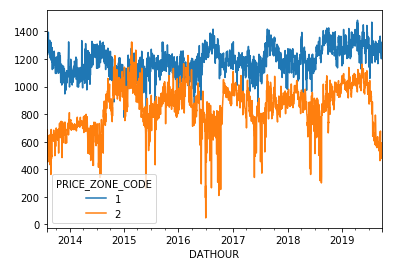
\includegraphics[width=5.4cm]{screenshot009}\hfil\hfil
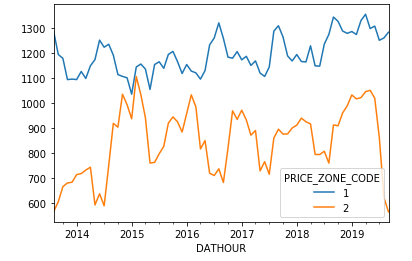
\includegraphics[width=5.6cm]{screenshot010}
\

Спотовые цены (усредненные за день/за месяц) для 1 и 2 ценовой зон, руб./МВт.ч

\begin{equation}\label{key}
corr(p_1^m,p_2^m)  =  0.07
\end{equation}


\end{frame}

%\begin{frame}[shrink=5]
%\frametitle{Российский оптовый рынок электричества} 
%\begin{figure}
%	\centering
%	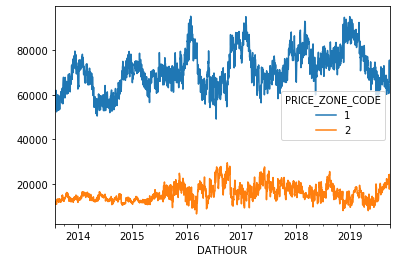
\includegraphics[width=0.7\linewidth]{screenshot011}
%	\caption{Разница дневных объемов планового предложения и потребления электроэнергии для 1 и 2 ценовой зон, МВт.ч.}
%	\label{fig:screenshot011}
%\end{figure}
%\end{frame}



\section{Факторы}




\begin{frame}[shrink=5]
\frametitle{Факторы  влияющие на цены на электричество} 
%\framesubtitle{Особенности рынка электричества} 

Особенности рынка электричества:
\begin{itemize}
	\item невозможность хранения $\rightarrow$ проблема обязательства энергоустановки (unit commitment); 
	\item проблема с ограничениями ЛЭП, возможность перенапряжения сети;
%	\item цены на электричество определяются на РСВ, т.е. отсутствует непрерывность торговли, решения на все сутки принимаются на основании одного и того же информационного множества
	\item невозможность перераспределить волатильность цен по производственной цепочке. 

\end{itemize}

Особенности российского рынка:

\begin{itemize}
	\item  высокая степень изношенности основных фондов  и потери тепла;
	
%\item  (*J) аварийность в электросетях и генерации, (ежемесячно или дамми на регионы с высокими рисками нарушения электроснабжения);
	%	https://minenergo.gov.ru/node/267
	% https://minenergo.gov.ru/node/989
	% https://minenergo.gov.ru/node/264
	% https://minenergo.gov.ru/node/11200
	%	высокая степень изношенности основных фондов
	
	
	
%	\item  Перекрестное субсидирование (частичный перенос платежного бремени с населения на промышленность).
	\item  проблема неплатежей; % (на конец октября 2017 года на оптовом рынке задолженность составила 65,2 млрд руб., а на розничном — 243 млрд руб).
	
%		\item  (*J) проблема неплатежей;
	
	
	\item  вынужденная генерация;  %(ТЭЦ  неэффективны на рынке электроэнергии, мощности, работающие в режиме вынужденной генерации, оплачиваются по существенно более высокой цене, чем рыночная).
	\item  завершение ДПМ и продление ДПМ ВИЭ.
	
%		\item  (**TJ) инвестиции в энергетику, завершение ДПМ и продление ДПМ ВИЭ;
%		\item  (*) доля ВИЭ и ГП, зависимых от погодных условий;
	
	
\end{itemize}

%	\item  (**TJ) структура генерирующих мощностей;
%	\item  (*J) государственная политика, новости;
%	\item  (***)   изменения в составе и правилах взаимодействия ценовых зон 
%   \item  (*S) коэффициенты сезонности, определенные АТС. %  цены имеют три уровня циклических колебаний: ежедневная, недельная, годовая (с резкими всплесками в январе)
%http://www.atsenergo.ru/sites/default/files/prognoz/20191128_ishodnye_dannye_i_prognoz_na_2020.pdf

\end{frame}





\begin{frame}[shrink=5]
\frametitle{Модель 1: выбор ценовых факторов} 
\begin{align*}
p_{t} = p_{ t-1} & + \mu + \beta_1 y_{t-1} + \beta_2 y_{t-7} + \beta_3 y_{t-30} +  \beta_4 y_{t-365} + \gamma_1 \hat{p}^{coal}_t +  \gamma_2 \hat{p}^{gas}_t  +  \\ &  +  \psi_1 T_{ t-1 } + \psi_2 T_{ t-30 } +  d_{ Sat} D_{ Sat,t} + d_{ Sun }D_{ Sun,t} + d_{ Mon }D_{ Mon,t} +  \\ & + \phi \mathbf{x}_t + \sqrt{exp(h_{ t-1} )}\epsilon_{ t }^{(1)}+ J _{t }\\
h_{t-1} &= h_{ t-2} + \kappa_{ h} (\theta_{ h} - h_{ t-2} ) + \sigma_{ h} (\rho \epsilon_{ t-1}^{(1)} + \sqrt{1 - \rho^2} \epsilon_{ t-1}^{(2)}) \\
J_{ t} &= -\xi_{ t}^D \cdot \mathbb{I}(q_{ t} = -1) + 0 \cdot \mathbb{I} (q_{ t} = 0) + \xi_{ t}^U \cdot \mathbb{I} (q_{ t} = 1)
\end{align*}
\footnotesize{
	\begin{itemize}
		\item $p_{ t} = ln(S_{ t})$ --  логарифм средней цены за день;
		\item  $y_{ t} = ln(Y_{ t})$ --  уровень деловой активности;   %  (ежедневной и общего тренда) (***TS)
		\item  $p^R_t$ -- логарифм прогноза цены на ресурсы, где $R = \{ coal, gas\}$; % + и инфляция;
		\item  $T_{ t}$ -- логарифм модуля средней дневной температуры (если  $\psi>0$, то большим отклонениям от нуля соответствуют большие цены);
		%  вчерашнее значение
		% или прогноз
		% или среднее за месяц (плавающее)
		
%			\item  (***S)   погодные условия; % погодные условия (причем при более точном прогнозировании погодных условий можно уменьшить ошибку прогноза цены на электричество)
		
		%	https://www.gismeteo.ru/diary/4517/2014/8/
		%	http://rpubs.com/lefkios_paikousis/weatherdata-in-r
		%https://rp5.ru/%D0%9F%D0%BE%D0%B3%D0%BE%D0%B4%D0%B0_%D0%B2_%D0%A0%D0%BE%D1%81%D1%81%D0%B8%D0%B8
		%https://cran.r-project.org/web/packages/rwunderground/rwunderground.pdf
		%https://blog.exploratory.io/riem-package-getting-world-weather-data-in-super-easy-way-78aa94ed45f5
		%http://aisori.meteo.ru/climater
		
		\item  $\mathbf{x}_t$  -- столбец других неценовых факторов, $\phi$ -- строка коэффициентов;
	
		\item  $D_{ Sat, t}, D_{ Sun, t}, D_{ Mon, t}$  -- учитывают недельную сезонность;
		
		\item  ненаблюдаемые переменные:  $h_{t-1} = p_{t} - p_{ t-1} = ln(S_{ t}/S_{ t-1} ) $ и  $q_{t}$ -- скачки вверх  ($\xi_{ t}^U \sim Exp(\eta_U) \ i.i.d. $) и вниз  ($\xi_{ t}^D \sim Exp(\eta_D) \ i.i.d. $);
		
		\item  $\rho$ -- параметр ''рычага'' ($\rho > 0$, если большим значениям логарифма цены  соответствуют большие значения дисперсии);
		$\epsilon_{ t }^{(1)}, \epsilon_{ t }^{(2)} \sim N(0,1) \ i.i.d.$.
		
		
		
		
	\end{itemize}
	
}

\end{frame}
























%\begin{frame}[shrink=5]
%\frametitle{Lucia and Schwartz (2002)} 
%
%Данные: 
%
%Nordic Power Exchange's спот-цены
%
%\begin{figure}
%	\centering
%	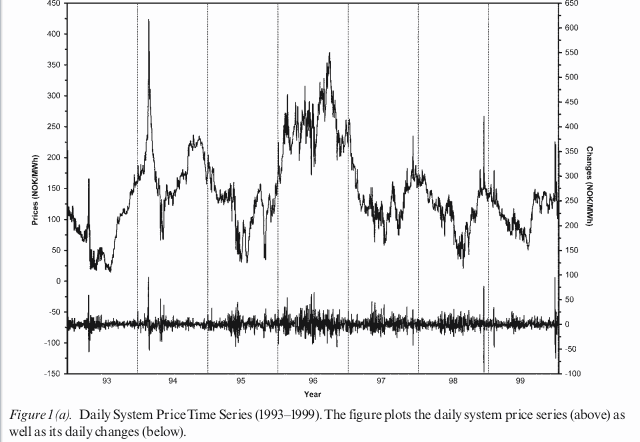
\includegraphics[width=0.7\linewidth]{screenshot007}
%	\caption{}
%	\label{fig:screenshot007}
%\end{figure}
%
%
%
%\end{frame}
%
%


%\begin{frame}[shrink=5]
%\frametitle{Cartea and Figueroa (2005) } 
%
%Модель: 
%
%Детерминистческая компонента - сезонность:
%
%$$\ln S_t = g(t) +Y_t$$
%
%Стохастическая компонента:
%
%$$dY_t = -\alpha Y_t dt + \sigma(t) dW_t + J dq_t$$
%
%$J$ - величина скачка, $q$ - пуассоновский процесс.
%
%
%\end{frame}

%
%\begin{frame}[shrink=5]
%\frametitle{Lucia and Schwartz (2002)} 
%
%Данные: 
%
%FTSE100; 2/01/90 - 18/06/04. 
%
%\begin{figure}
%	\centering
%	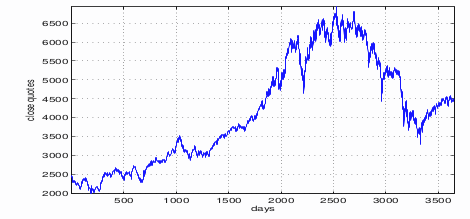
\includegraphics[width=0.7\linewidth]{screenshot008}
%	\caption{}
%	\label{fig:screenshot008}
%\end{figure}
%
%
%
%\end{frame}
















\section{Приложения}

%
%\begin{frame}[shrink=5]
%\frametitle{Приложение A.1} 
%\framesubtitle{Российский оптовый рынок электричества} 
%\begin{figure}
%	\centering
%	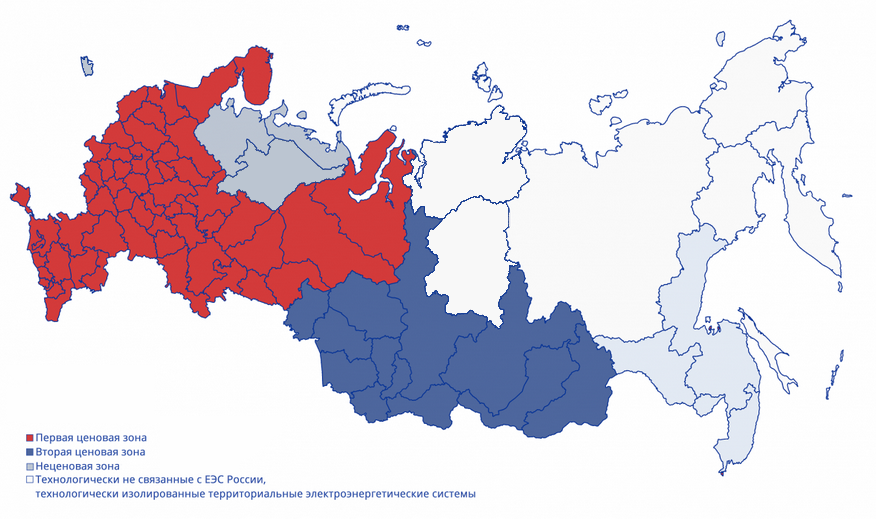
\includegraphics[width=1\linewidth]{screenshot014}
%	\caption{ Ценовые зоны. Источник: АТС }
%	\label{fig:screenshot013}
%\end{figure}
%\end{frame}

\begin{frame}[shrink=5]
\frametitle{Приложение A} 
\framesubtitle{Российский оптовый рынок электричества} 
\begin{figure}
\centering
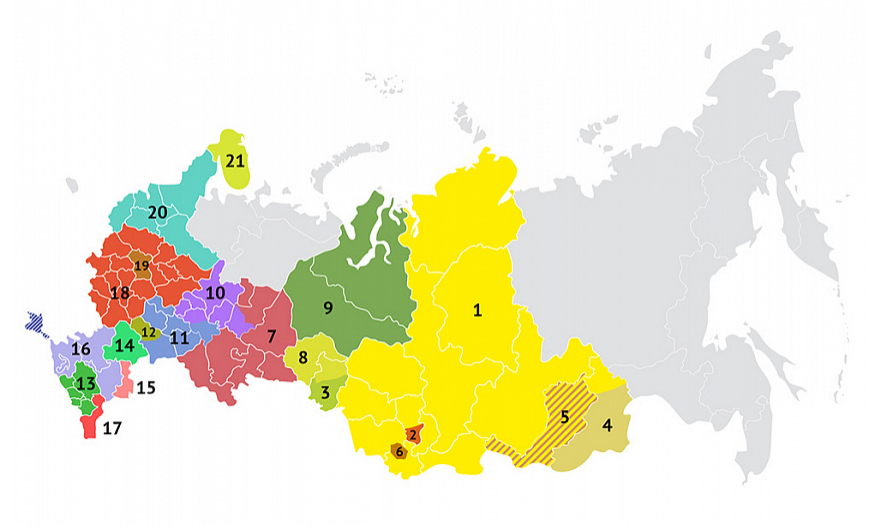
\includegraphics[width=0.7\linewidth]{screenshot16}
\caption{ Зоны свободного перетока мощности оптового рынка.  Источник: ПЕРЕТОК.РУ }
\label{fig:screenshot015}
\end{figure}
%https://peretok.ru/articles/strategy/14495/
\footnotesize{* С точки зрения энергорынка, разделение на ЗСП по-прежнему учитывается только при определении вынужденной генерации, при этом используется базовый перечень ЗСП.}
\end{frame}


\begin{frame}[shrink=5]
\frametitle{Приложение Б.1} 
\framesubtitle{Регламент проведения конкурентного  отбора заявок для балансирования системы} 

\footnotesize{
\begin{itemize}
	\item При формировании поузловых модельных пар <цена-количество> СО  определяет на основе ценовых заявок на планирование объемов производства в отношении групп точек поставки (ГТП) генерации объемы электрической энергии, заявленные Участниками оптового рынка в отношении каждой ГТП генерации к продаже на сутки вперед, и из этих объемов выделяет объемы (часть объемов) электрической энергии, и формирует на эти объемы ценопринимающую часть вместо условий третьего и четвертого приоритета для модельных пар;
	\item если ГТП относится к нескольким узлам расчетной модели, СО распределяет объемы электрической энергии, содержащиеся в каждой паре «цена – количество» в ценовой заявке в соответствии с коэффициентами или формулами отнесения объемов к каждому узлу;
	\item  пределы регулирования (Рмин и Рмакс) определяются для ГТП генерации и объектов управления, относящихся к ГТП потребления с регулируемой нагрузкой, с разделением по техническим и технологическим (с учетом вынужденных режимов и ограничений по топливу) характеристикам, причинам поддержания регулировочного резерва мощности в системе.
\end{itemize}
}

\end{frame}



\begin{frame}[shrink=5]
\frametitle{Приложение Б.2} 
\framesubtitle{Регламент проведения конкурентного  отбора заявок для балансирования системы} 

\footnotesize{
СО проводит конкурентный отбор БР и определение диспетчерских объемов, индикаторов стоимости и цен балансирования в соответствии с Математической моделью расчета диспетчерских объемов электрической энергии, индикаторов и цен на балансирование вверх (вниз) в результате конкурентного отбора ценовых заявок БР так, чтобы:
}
\begin{itemize}
\item в диспетчерские объемы были включены все объемы электрической энергии, не превышающие установленных пределов, относящиеся к соответствующему узлу;
\item индикатор в данном узле был не меньше цены, указанной Участником оптового рынка в ценовой заявке на планирование объема отрицательного потребления в отношении ГТП потребления с регулируемой нагрузкой по объекту управления или в ценовой заявке на планирование объема производства в отношении ГТП генерации за объем электрической энергии;
\item индикаторы во всех узлах расчетной модели отличались на стоимость нагрузочных потерь электрической энергии и системных ограничений.
\end{itemize}
\end{frame}


\begin{frame}[shrink=5]
\frametitle{Приложение Б.3} 
\framesubtitle{Специальные случаи расчета результатов конкурентного отбора} 

\footnotesize{
Если при проведении конкурентного отбора БР для определенного операционного часа в некоторой группе узлов расчетной модели:

\begin{itemize}
\item  приняты только ценопринимающие объемы в заявках на продажу индикаторы в этой группе узлов считаются равными нулю;
\item принята заявка с четвертой (дополнительной) ступенью, с ценой или с модельной ценой, равной десяти тарифам на электроэнергию, для определения индикаторов стоимости на данный час проводится дополнительный расчет, обеспечивающий вычисление индикаторов стоимости по ценам, не превышающих указанной модельной цены и максимальной из цен, указанных в принятых третьих ступенях ценовых заявок участников;
\item  оказывается, что для какого-либо часа объемов производства недостаточно для формирования ПБР, удовлетворяющего в этот час остальным СО вправе изменить состав выбранного оборудования;
\item 	 не удается выполнить действия предыдущего подпункта  СО имеет право в установленном порядке ввести ограничения потребления и/или изменить ограничения на перетоки по сечениям экспортно-импортных операций.
\end{itemize}
}

\end{frame}



\begin{frame}[shrink=5]
\frametitle{Приложение B.1} 
\framesubtitle{Параметры спроса и предложения электрической энергии} 

Ценовая зона --  Европа 

Дата: 12.07.2018. 10:00 


\begin{table}[]
	\begin{tabular}{l|ll|ll}
		 & ЦЗ на покупку &  & ЦЗ на продажу &  \\
		& Цена, руб./МВтч & Объем, МВтч & Цена, руб./МВтч & Объем, МВтч \\\hline\hline
		1 & * & 88253.36 & * & 83264.25 \\\hline
		2 & 100 & 1 & 271 & 3 \\\hline
		3 & 1900 & 33.705 & 300 & 54 \\
		4 & 2300 & 41 & 390 & 0.9999 \\\hline
		5 &  &  & 427 & 1 \\
		6 &  &  & 429 & 49.66 \\
		7 &  &  & 444 & 1 \\
		… &  &  & … & … \\
		208 &  &  & 3000 & 32 \\
		209 &  &  & 3500 & 0.5 \\
		210 &  &  & 3860 & 4.375 \\
		211 &  &  & 5490 & 27 \\
		212 &  &  & 5842 & 2 \\
		213 &  &  & 6100 & 9.5 \\
		214 &  &  & 13260 & 102.652\\\hline
	\end{tabular}
\end{table}

(*) -- заявки ценополучателей

Источник: АТС

\end{frame}

%
%\begin{frame}[shrink=5]
%\frametitle{Приложение B.2} 
%\framesubtitle{Плановые почаcовые объемы потребления} 
%
%
%Плановые почаcовые объемы потребления, МВтЧ.: 
%
%\begin{table}[]
%\begin{tabular}{llllll}
%	Дата & 17.07.2019 &  &  &  &  \\
%	ЦЗ: & Европа &  &  &  &  \\
%	&  &  &  &  &  \\
%	Час &  &  &  &  &  \\
%	& … & 11-12 & 12-13 & 13-14 & … \\
%	ГП & … & 52507.568 & 52146.723 & 52444.545 & … \\
%	не ГП & … & 31586.293 & 31625.01 & 31707.908 & …
%\end{tabular}
%\end{table}
%
%Источник: АТС
%
%
%\
%
%\footnotesize{* Гарантирующий поставщик обязан заключить с любым обратившимся к нему физическим или юридическим лицом, находящимся в зоне его деятельности, договор энергоснабжения (купли-продажи (поставки) электрической энергии (мощности)).
%}
%
%
%\end{frame}
%
%


\begin{frame}[shrink=5]
\frametitle{Приложение B.2} 
\framesubtitle{Модель расчета узловых цен} 

\begin{figure}
\centering
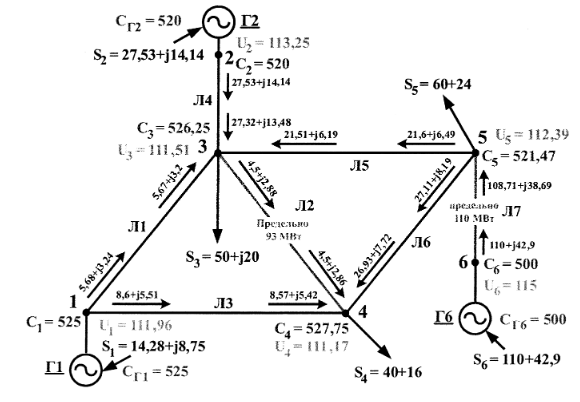
\includegraphics[width=0.8\linewidth]{screenshot022}
\caption{ Математическая модель расчета узловых цен по методике АТС. Источник: Б.Г. Булатов, В.О. Каркунов (2009)  }
\label{fig:screenshot015}
\end{figure}


%https://www.mbureau.ru/tag/uzlovye-ceny

\end{frame}







\section{Risks}


\section{Derivatives}


\section{Estimation}



%
%
%\begin{frame}[shrink=5]
%\frametitle{Данные} 
%
%
%
%
%\begin{figure}
%	\centering
%	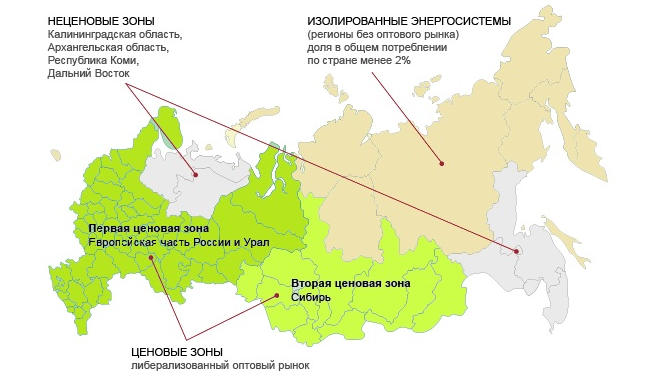
\includegraphics[width=0.7\linewidth]{screenshot003}
%	\caption{ Ценовые зоны  }
%	\label{fig:screenshot003}
%\end{figure}
%
%\end{frame}
%
%

%
%
%\begin{frame}[shrink=5]
%\frametitle{Данные} 
%
%
%
%
%
%\begin{figure}
%	\centering
%	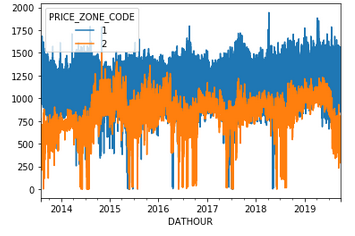
\includegraphics[width=0.7\linewidth]{screenshot002}
%	\caption{ Почасовые цены в первой и второй ценовых зонах }
%	\label{fig:screenshot002}
%\end{figure}
%
%\end{frame}

%\begin{frame}[shrink=5]
%\frametitle{Специфика российского рынка} 
%
%Примеры:
%
%\begin{itemize}
%	\item 29.03.09 на  фоне снижения спроса отмечено увеличение перетока по контролируемому сечению между ценовыми зонами в сторону Сибири. Отмечено снижение цены в ценовых заявках поставщиков  => принято предложение по наиболее низким ценам 
%	\item   3.06.09 резкое падение индекса равновесных цен по причине снижения спроса на ээ => замыкающими оказались низкие ценовые заявки 
%	\item  13.09.09 снижение потребления электроэнергии вследствие отсутствия заявки на покупку со стороны одного из крупных потребителей => индекс цен снизился
%	
%\end{itemize}
%
%
%\end{frame}
%
%







\end{document}